% (find-LATEX "2021-1-C3-MT1.tex")
% (defun c () (interactive) (find-LATEXsh "lualatex -record 2021-1-C3-MT1.tex" :end))
% (defun C () (interactive) (find-LATEXsh "lualatex 2021-1-C3-MT1.tex" "Success!!!"))
% (defun D () (interactive) (find-pdf-page      "~/LATEX/2021-1-C3-MT1.pdf"))
% (defun d () (interactive) (find-pdftools-page "~/LATEX/2021-1-C3-MT1.pdf"))
% (defun e () (interactive) (find-LATEX "2021-1-C3-MT1.tex"))
% (defun o () (interactive) (find-LATEX "2021-1-C3-MT1.tex"))
% (defun u () (interactive) (find-latex-upload-links "2021-1-C3-MT1"))
% (defun v () (interactive) (find-2a '(e) '(d)))
% (defun d0 () (interactive) (find-ebuffer "2021-1-C3-MT1.pdf"))
% (defun cv () (interactive) (C) (ee-kill-this-buffer) (v) (g))
%          (code-eec-LATEX "2021-1-C3-MT1")
% (find-pdf-page   "~/LATEX/2021-1-C3-MT1.pdf")
% (find-sh0 "cp -v  ~/LATEX/2021-1-C3-MT1.pdf /tmp/")
% (find-sh0 "cp -v  ~/LATEX/2021-1-C3-MT1.pdf /tmp/pen/")
%     (find-xournalpp "/tmp/2021-1-C3-MT1.pdf")
%   file:///home/edrx/LATEX/2021-1-C3-MT1.pdf
%               file:///tmp/2021-1-C3-MT1.pdf
%           file:///tmp/pen/2021-1-C3-MT1.pdf
% http://angg.twu.net/LATEX/2021-1-C3-MT1.pdf
% (find-LATEX "2019.mk")
% (find-CN-aula-links "2021-1-C3-MT1" "3" "c3m211mt1" "c3mt1")
%
% Video (not yet):
% (find-ssr-links "c3m211mt1" "2021-1-C3-MT1")
% (code-video     "c3m211mt1video" "$S/http/angg.twu.net/eev-videos/2021-1-C3-MT1.mp4")
% (find-c3m211mt1video "0:00")

% «.defs»		(to "defs")
% «.title»		(to "title")
% «.introducao»		(to "introducao")
% «.introducao-2»	(to "introducao-2")
% «.links»		(to "links")
%
% «.djvuize»	(to "djvuize")

\documentclass[oneside,12pt]{article}
\usepackage[colorlinks,citecolor=DarkRed,urlcolor=DarkRed]{hyperref} % (find-es "tex" "hyperref")
\usepackage{amsmath}
\usepackage{amsfonts}
\usepackage{amssymb}
\usepackage{pict2e}
\usepackage[x11names,svgnames]{xcolor} % (find-es "tex" "xcolor")
\usepackage{colorweb}                  % (find-es "tex" "colorweb")
%\usepackage{tikz}
%
% (find-dn6 "preamble6.lua" "preamble0")
%\usepackage{proof}   % For derivation trees ("%:" lines)
%\input diagxy        % For 2D diagrams ("%D" lines)
%\xyoption{curve}     % For the ".curve=" feature in 2D diagrams
%
\usepackage{edrx21}               % (find-LATEX "edrx21.sty")
\input edrxaccents.tex            % (find-LATEX "edrxaccents.tex")
\input edrxchars.tex              % (find-LATEX "edrxchars.tex")
\input edrxheadfoot.tex           % (find-LATEX "edrxheadfoot.tex")
\input edrxgac2.tex               % (find-LATEX "edrxgac2.tex")
%
%\usepackage[backend=biber,
%   style=alphabetic]{biblatex}            % (find-es "tex" "biber")
%\addbibresource{catsem-slides.bib}        % (find-LATEX "catsem-slides.bib")
%
% (find-es "tex" "geometry")
\usepackage[a6paper, landscape,
            top=1.5cm, bottom=.25cm, left=1cm, right=1cm, includefoot
           ]{geometry}
%
\begin{document}

%\catcode`\^^J=10
%\directlua{dofile "dednat6load.lua"}  % (find-LATEX "dednat6load.lua")

% %L dofile "edrxtikz.lua"  -- (find-LATEX "edrxtikz.lua")
% %L dofile "edrxpict.lua"  -- (find-LATEX "edrxpict.lua")
% \pu

% «defs»  (to ".defs")
% (find-LATEX "edrx15.sty" "colors-2019")
%\long\def\ColorRed   #1{{\color{Red1}#1}}
%\long\def\ColorViolet#1{{\color{MagentaVioletLight}#1}}
%\long\def\ColorViolet#1{{\color{Violet!50!black}#1}}
%\long\def\ColorGreen #1{{\color{SpringDarkHard}#1}}
%\long\def\ColorGreen #1{{\color{SpringGreenDark}#1}}
%\long\def\ColorGreen #1{{\color{SpringGreen4}#1}}
%\long\def\ColorGray  #1{{\color{GrayLight}#1}}
%\long\def\ColorGray  #1{{\color{black!30!white}#1}}
%\long\def\ColorBrown #1{{\color{Brown}#1}}
%\long\def\ColorBrown #1{{\color{brown}#1}}
%\long\def\ColorOrange#1{{\color{orange}#1}}
%
%\long\def\ColorShort #1{{\color{SpringGreen4}#1}}
%\long\def\ColorLong  #1{{\color{Red1}#1}}
%
%\def\frown{\ensuremath{{=}{(}}}
%\def\True {\mathbf{V}}
%\def\False{\mathbf{F}}
%\def\D    {\displaystyle}

\def\drafturl{http://angg.twu.net/LATEX/2021-1-C3.pdf}
\def\drafturl{http://angg.twu.net/2021.1-C3.html}
\def\draftfooter{\tiny \href{\drafturl}{\jobname{}} \ColorBrown{\shorttoday{} \hours}}



%  _____ _ _   _                               
% |_   _(_) |_| | ___   _ __   __ _  __ _  ___ 
%   | | | | __| |/ _ \ | '_ \ / _` |/ _` |/ _ \
%   | | | | |_| |  __/ | |_) | (_| | (_| |  __/
%   |_| |_|\__|_|\___| | .__/ \__,_|\__, |\___|
%                      |_|          |___/      
%
% «title»  (to ".title")
% (c3m211mt1p 1 "title")
% (c3m211mt1a   "title")

\thispagestyle{empty}

\begin{center}

\vspace*{1.2cm}

{\bf \Large Cálculo 3 - 2021.1}

\bsk

Mini-teste 1

\bsk

Eduardo Ochs - RCN/PURO/UFF

\url{http://angg.twu.net/2021.1-C3.html}

\end{center}

\newpage

% «introducao»  (to ".introducao")
% (c3m211mt1p 2 "introducao")
% (c3m211mt1a   "introducao")

{\bf Introdução}

Em $\R^2$ nós sabemos levantar pontos do eixo $x$ pra uma curva
$y=f(x)$, e sabemos projetar estes pontos no eixo vertical...

% (find-latexscan-links "C3" "20210723_x0x1y0y1")
% (find-xpdf-page "~/LATEX/2021-1-C3/20210723_x0x1y0y1.pdf")
$$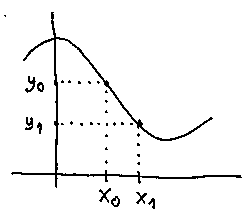
\includegraphics[height=4cm]{2021-1-C3/20210723_x0x1y0y1.pdf}$$

...e também sabemos projetar esses pontos numa reta tangente à nossa
curva $y=f(x)$, mas aí tanto as contas quanto os desenhos são mais
complicados.

\newpage

% «introducao-2»  (to ".introducao-2")
% (c3m211mt1p 3 "introducao-2")
% (c3m211mt1a   "introducao-2")

{\bf Introdução (2)}

O passo seguinte é aprendermos a fazer algo parecido com trajetórias e
superfícies em $\R^3$, e usando planos tangentes além de retas
tangentes. Os desenhos vão ficar bem mais complicados, as contas
também, e as contas vão ficar praticamente impossíveis de entender se
a gente não souber visualizar o que elas querem dizer.

Eu preciso que vocês comecem a fazer os desenhos de vocês, e comecem a
praticar isso bastante. Eu não conheço nenhum lugar -- livro, artigo,
site, o que for -- que ensine direito as técnicas pra fazer os
desenhos que a gente precisa fazer em C3 de um jeito que os desenhos
fiquem claros, então estou tendo que inventar um jeito de ensinar
isso. A gente vai começar vendo os tipos de desenhos que as pessoas
aprenderam a fazer em C3 no semestre passado, mas dessa vez um jeito
bem mais organizado, e agora cada técnica que a gente vai usar vai ter
nome.

\newpage

% «links»  (to ".links")
% (c3m211mt1p 4 "links")
% (c3m211mt1a   "links")

{\bf Links}

Alguns links pra desenhos que aprendemos

a usar e a fazer no semestre passado:

\msk

Cortes no olhômetro numa superfície curva:

{\footnotesize

% (c3m202mt1p 4 "figura-intro")
% (c3m202mt1a   "figura-intro")
% (c3m202rcadeia1p 27 "figura-thomas")
% (c3m202rcadeia1a    "figura-thomas")

\url{http://angg.twu.net/LATEX/2020-2-C3-MT1.pdf#page=4}

\url{http://angg.twu.net/LATEX/2020-2-C3-rcadeia1.pdf#page=27}

}

\msk

Tem vários desenhos no PDF sobre plano tangente --

veja principalmente as páginas 10, 23 e da 27 em diante...

{\footnotesize

% (c3m202planotangp 10 "geral-e-particular")
% (c3m202planotang     "geral-e-particular")
% (c3m202planotangp 23 "derivs-como-triangs-2")
% (c3m202planotanga    "derivs-como-triangs-2")

\url{http://angg.twu.net/LATEX/2020-2-C3-plano-tang.pdf#page=10}

\url{http://angg.twu.net/LATEX/2020-2-C3-plano-tang.pdf#page=23}

}

\msk

Leia a ``Dica 7'', que é sobre desenhos feitos pra você mesmo,

desenhos feitos pra um colega que seja seu amigo, e desenhos

feitos pra que todo mundo entenda...

{\footnotesize

% (c2m211somas1dp 7 "dica-7")
% (c2m211somas1da   "dica-7")

\url{http://angg.twu.net/LATEX/2021-1-C2-somas-1-dicas.pdf#page=7}

}


% (c3p1p 9 "gabarito-1f")
% (c3p1a   "gabarito-1f")


\newpage


Este mini-teste vai ser sobre desenhos ainda mais básicos

do que os dos links da página anterior. As questões vão ser

baseadas nas questões daqui:

\ssk

{\footnotesize

% http://angg.twu.net/LATEX/2021-1-C3-planos.pdf
\url{http://angg.twu.net/LATEX/2021-1-C3-planos.pdf}

}

\bsk

As regras vão ser as mesmas dos

mini-testes do semestre passado:

\ssk

{\footnotesize

\url{http://angg.twu.net/LATEX/2020-2-C2-MT1.pdf#page=2}

}

(Leia com muita atenção!!!!!!!!!!!)

\bsk

As questões vão ser disponibilizadas às 20:00 da sexta

23/julho/2021 e vocês vão ter até as 20:00 do sábado

24/julho/2021 pra entregar as respostas.



\newpage

{\bf Questão 1}

(0.2 pts) Sejam:
%
$$\begin{array}{rcl}
  π_1 &=& [z=1], \\
  π_2 &=& [x+y=3], \\
  r &=& π_1∩π_2, \\
  \end{array}
$$

e sejam $A$ e $B$ dois pontos da reta $r$ ---

que você vai escolher e dizer as coordenadas deles.

\msk

Represente graficamente $π_1$, $π_2$, $r$, $A$ e $B$.

\msk

Lembre que o desafio principal é fazer desenhos

que fiquem muito claros e legíveis!


\newpage

{\bf Questão 2}

\def\psiii#1{(#1)_{Σ_3}}
\def\psiv #1{(#1)_{Σ_4}}

(0.3 pts) Sejam:
%
$$\begin{array}{rcl}
  \psiii{a,b} &=& (3,1,1) + a\VEC{1,0,0}  + b\VEC{0,1,0}, \\
  \psiv {c,d} &=& (2,1,3) + c\VEC{-1,1,0} + d\VEC{0,0,1}, \\
  π_3 &=& \setofst{\psiii{a,b}}{a,b∈\R} \\
  π_4 &=& \setofst{\psiv {c,d}}{c,d∈\R} \\
  \end{array}
$$

Represente graficamente, se possível num desenho só:

a) $\psiii{0,0}$, $\psiii{1,0}$, $\psiii{0,1}$, 

b) $\psiv {0,0}$, $\psiv {1,0}$, $\psiv {0,1}$, 

c) os planos $π_3$ e $π_4$,

d) os pontos $\psiii{-2,1}$ e $\psiv{1,-2}$.

\newpage

\vspace*{-0.7cm}

{\bf Dicas pra questão 2}

\msk

Depois de fazer os itens a e b você deve ser capaz

de descobrir os planos $π_3$ e $π_4$ no olhômetro, já que

você já tem três pontos de cada um.

\msk

Dê nomes curtos para os pontos $(3,1,1)$

e $(2,1,3)$ e para os quatro vetores.

\msk

Desenhe os vetores que você acha que podem

deixar o seu desenho mais fácil de entender.

\msk

Escreva quantas coisas do lado do seu desenho

quanto você quiser.

\msk

Se você quiser fazer uma anotação do lado de

um ponto ou vetor mas você achar que a anotação

é grande demais você pode escrever ela mais

longe e usar uma seta.







%\printbibliography

\GenericWarning{Success:}{Success!!!}  % Used by `M-x cv'

\end{document}

%  ____  _             _         
% |  _ \(_)_   ___   _(_)_______ 
% | | | | \ \ / / | | | |_  / _ \
% | |_| | |\ V /| |_| | |/ /  __/
% |____// | \_/  \__,_|_/___\___|
%     |__/                       
%
% «djvuize»  (to ".djvuize")
% (find-LATEXgrep "grep --color -nH --null -e djvuize 2020-1*.tex")

 (eepitch-shell)
 (eepitch-kill)
 (eepitch-shell)
# (find-fline "~/2021.1-C3/")
# (find-fline "~/LATEX/2021-1-C3/")
# (find-fline "~/bin/djvuize")

cd /tmp/
for i in *.jpg; do echo f $(basename $i .jpg); done

f () { rm -fv $1.png $1.pdf; djvuize $1.pdf }
f () { rm -fv $1.png $1.pdf; djvuize WHITEBOARDOPTS="-m 1.0" $1.pdf; xpdf $1.pdf }
f () { rm -fv $1.png $1.pdf; djvuize WHITEBOARDOPTS="-m 0.5" $1.pdf; xpdf $1.pdf }
f () { rm -fv $1.png $1.pdf; djvuize WHITEBOARDOPTS="-m 0.25" $1.pdf; xpdf $1.pdf }
f () { cp -fv $1.png $1.pdf       ~/2021.1-C3/
       cp -fv        $1.pdf ~/LATEX/2021-1-C3/
       cat <<%%%
% (find-latexscan-links "C3" "$1")
%%%
}

f 20210723_x0x1y0y1



%  __  __       _        
% |  \/  | __ _| | _____ 
% | |\/| |/ _` | |/ / _ \
% | |  | | (_| |   <  __/
% |_|  |_|\__,_|_|\_\___|
%                        
% <make>

 (eepitch-shell)
 (eepitch-kill)
 (eepitch-shell)
# (find-LATEXfile "2019planar-has-1.mk")
make -f 2019.mk STEM=2021-1-C3-MT1 veryclean
make -f 2019.mk STEM=2021-1-C3-MT1 pdf

% Local Variables:
% coding: utf-8-unix
% ee-tla: "c3mt1"
% ee-tla: "c3m211mt1"
% End:
